Support vector machines (SVM) can be used for forecasting in the commodity market. In \cite{xie2006new} they use SVMs for predicting the crude oil prices. SVMs are by nature a linear learning machine which means SVMs always use linear functions to solve the regression analysis but they can be expanded to be able to solve nonlinear problems. This is done by mapping the data into a high-dimensional feature space using a nonlinear mapping and then using the linear regression on this space. The SVMs undergo four different phases before being able to make the prediction. These can be seen in figure ~\ref{fig:phasesOfSVM}
\begin{figure}[weight!]
\centering
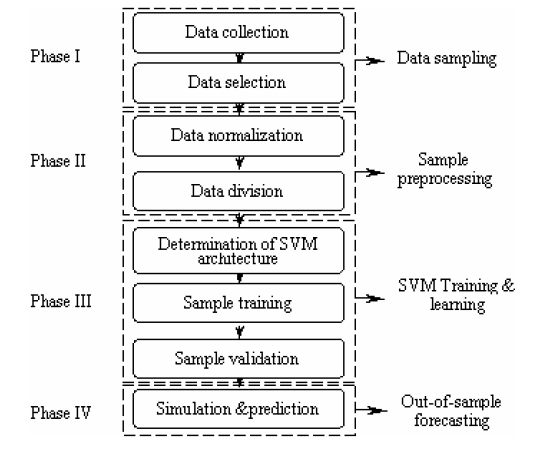
\includegraphics[width=0.8\textwidth ,natwidth=410,natheight=237]{billeder/phases_of_SVM.png}
\caption{The steps taken to create a Support Vector Machine}
\label{fig:phasesOfSVM}
\end{figure}
Data sampling is done daily but due to inconsistencies in these data they adopt weekly and monthly data as alternatives. Data preprocessing is done by transforming the data appropriate for learning. This can be done by using logarithmic transformation. The training and learning step is used for determining the architecture and the parameters of the SVM. There is no criterion for deciding this other than just trail-and-error. Out-of-sample forecasting is done on new data and the prediction is made. As for evaluation they use the Root Mean Square Error (RMSE) to describe the estimates deviations from the real values. Their results and analysis shows that their SVM performs better than both ARIMA and Back Propagation Neural Networks (In most cases). They argue that SVMs gives better predictions than ARIMA and BPNNs in most cases but neural networks might perform better with data that is optimized for neural networks. Also the neural network outperforms the SVM in one of their sub-period comparisons.

SVMs have also been used for load forecasting of electricity demand. In \cite{chen2004load} they use SVMs to make short-term predictions such as one-day ahead predictions. The goal of this study was to win a competition held by the EUNITE (EUropean Network on Intelligent TEchnologies for Smart Adaptive Systems). This was the winning proposal in the competition. They first examined the data which was half-hourly load demand recorded from 1997 to 1998. They figured out that in the wintertime load demand was higher than in the summertime thus indicating a connection to weather data. The weekends could also be separated from the weekdays since the weekend load was lower than regular weekdays. When analysis was done they started setting up the model. First of all they prepare the data and select the data needed for the prediction. They select calendar attributes to map the holidays and which day it is to account for lower demands. Temperature is included in the vectors used for prediction of the electricity load demand and historical data is incorporated as well. The data segmentation in the steps of preparing a SVM allows them to take only a subset of the data since most of it can be generalized in the data analysis thus making it easier to do computations. They argue that their model for forecasting demand loads are the best possible model used in this competition and to give a more varied view on this they try out other methods among these Neural Networks. They configure a neural network that first performs work on the same data as their Support Vector Machine and it provides less than satisfactory feedback with an error margin of 6-8\%. If they take the basic values used in the competition without doing any precomputation on it they receive a much better result of 3.64\%. From this they conclude that their SVM is performing better than Neural Networks in the specific problem and that neural networks performance depends mainly on what data you use as input. 